To guarantee the service required in \autoref{sec:problem_description}, different orbits have been taken in account.
The most used orbit to ensure a stable and reliable satellite communication is Geostationary.
\autoref{fig:GEOCoverage} has been taken from the Inmarsat's Website, and shown as a GEO satellite can not reach the latitudes over $75^\circ$. 

\begin{figure}
	\centering
	\begin{minipage}{0.45\textwidth}
		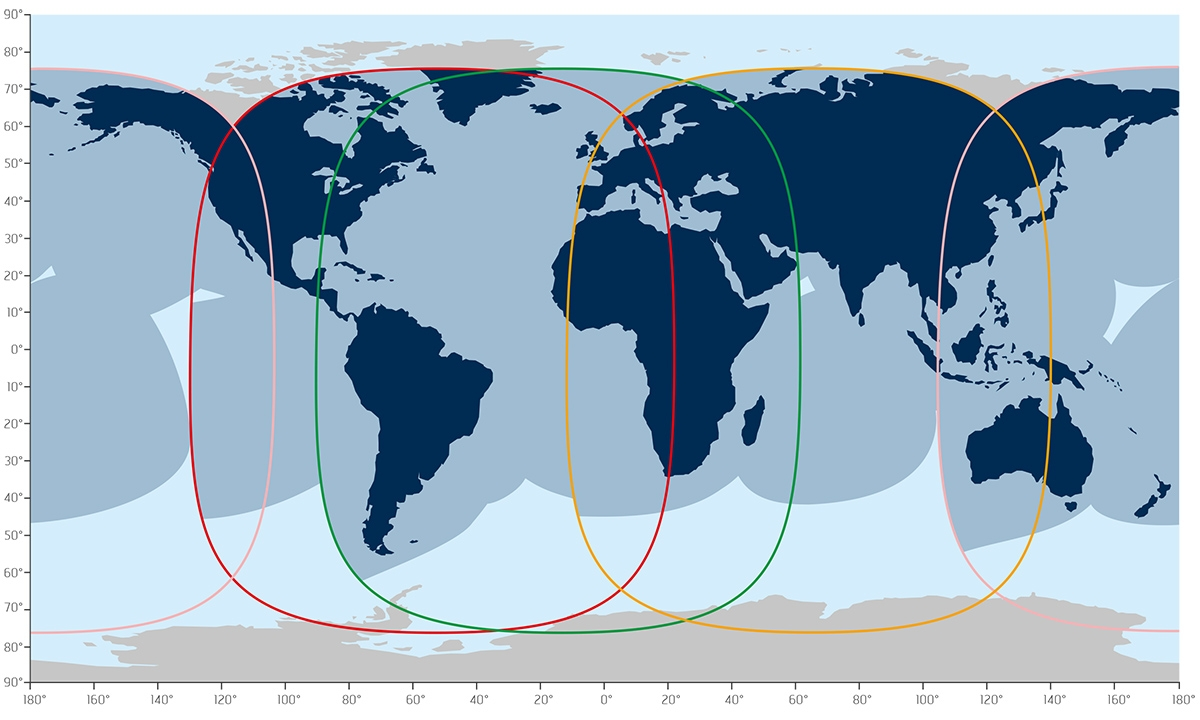
\includegraphics[width=\textwidth]{figures/GEOCoverage.jpeg}
		\caption{Approximate coverage of GEO Satellites.}
		\label{fig:GEOCoverage}
	\end{minipage}\hspace{0.5cm}
	\begin{minipage}{0.45\textwidth}
		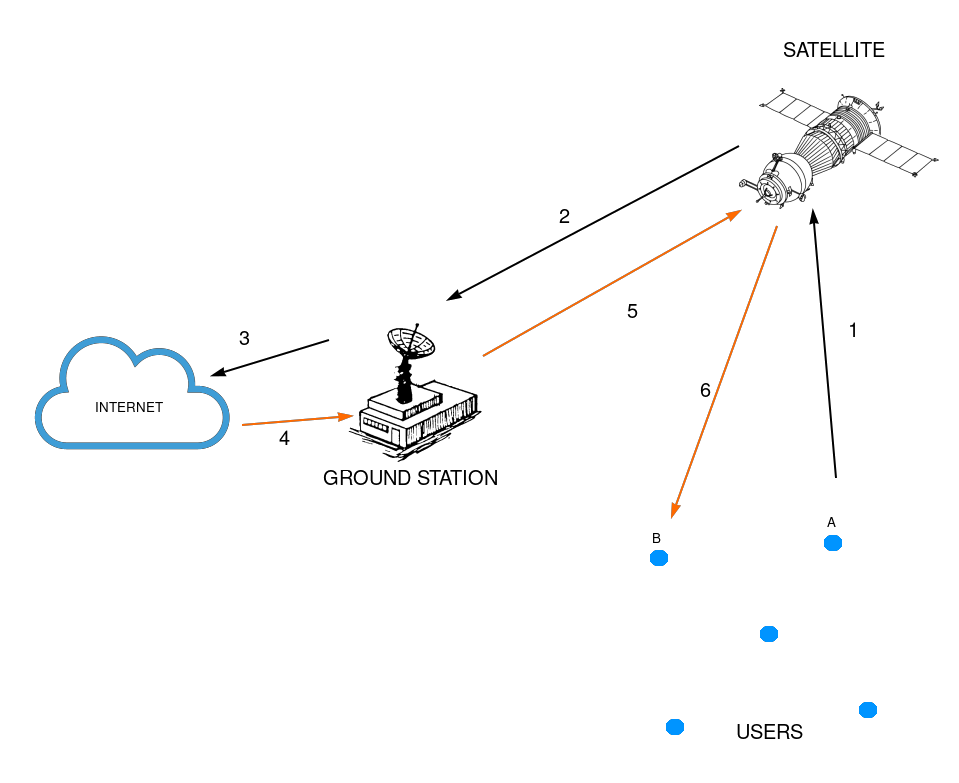
\includegraphics[width=\textwidth]{figures/System_topology_noBG.png}
		\caption{Typical communication path between an user A and an user B.}
	\end{minipage}
\end{figure}
